%!TEX root = 2017-icip-provenance-filtering.tex
\section{Introduction and Related Work}
\label{sec:intro}
%
\begin{figure}[htb]
	\begin{center}
	\subfigure[Semantically-similar \& near-duplicate images.\label{provenance_nndr}]{
		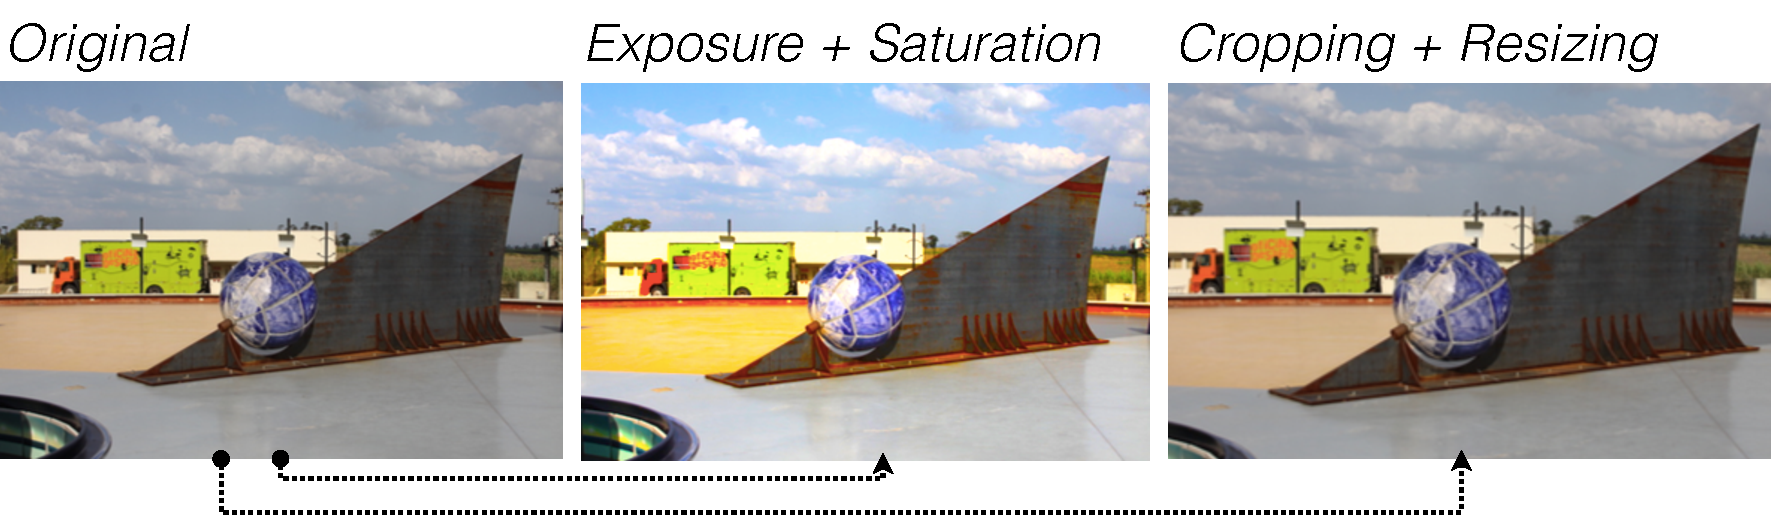
\includegraphics[width=0.67\columnwidth]{montage-provenance-filtering-01}
	}
	\subfigure[Multiple parenting multimedia phylogeny setup with an image composition and its several ancestors (donors)\label{provenance_mpp}.]{
		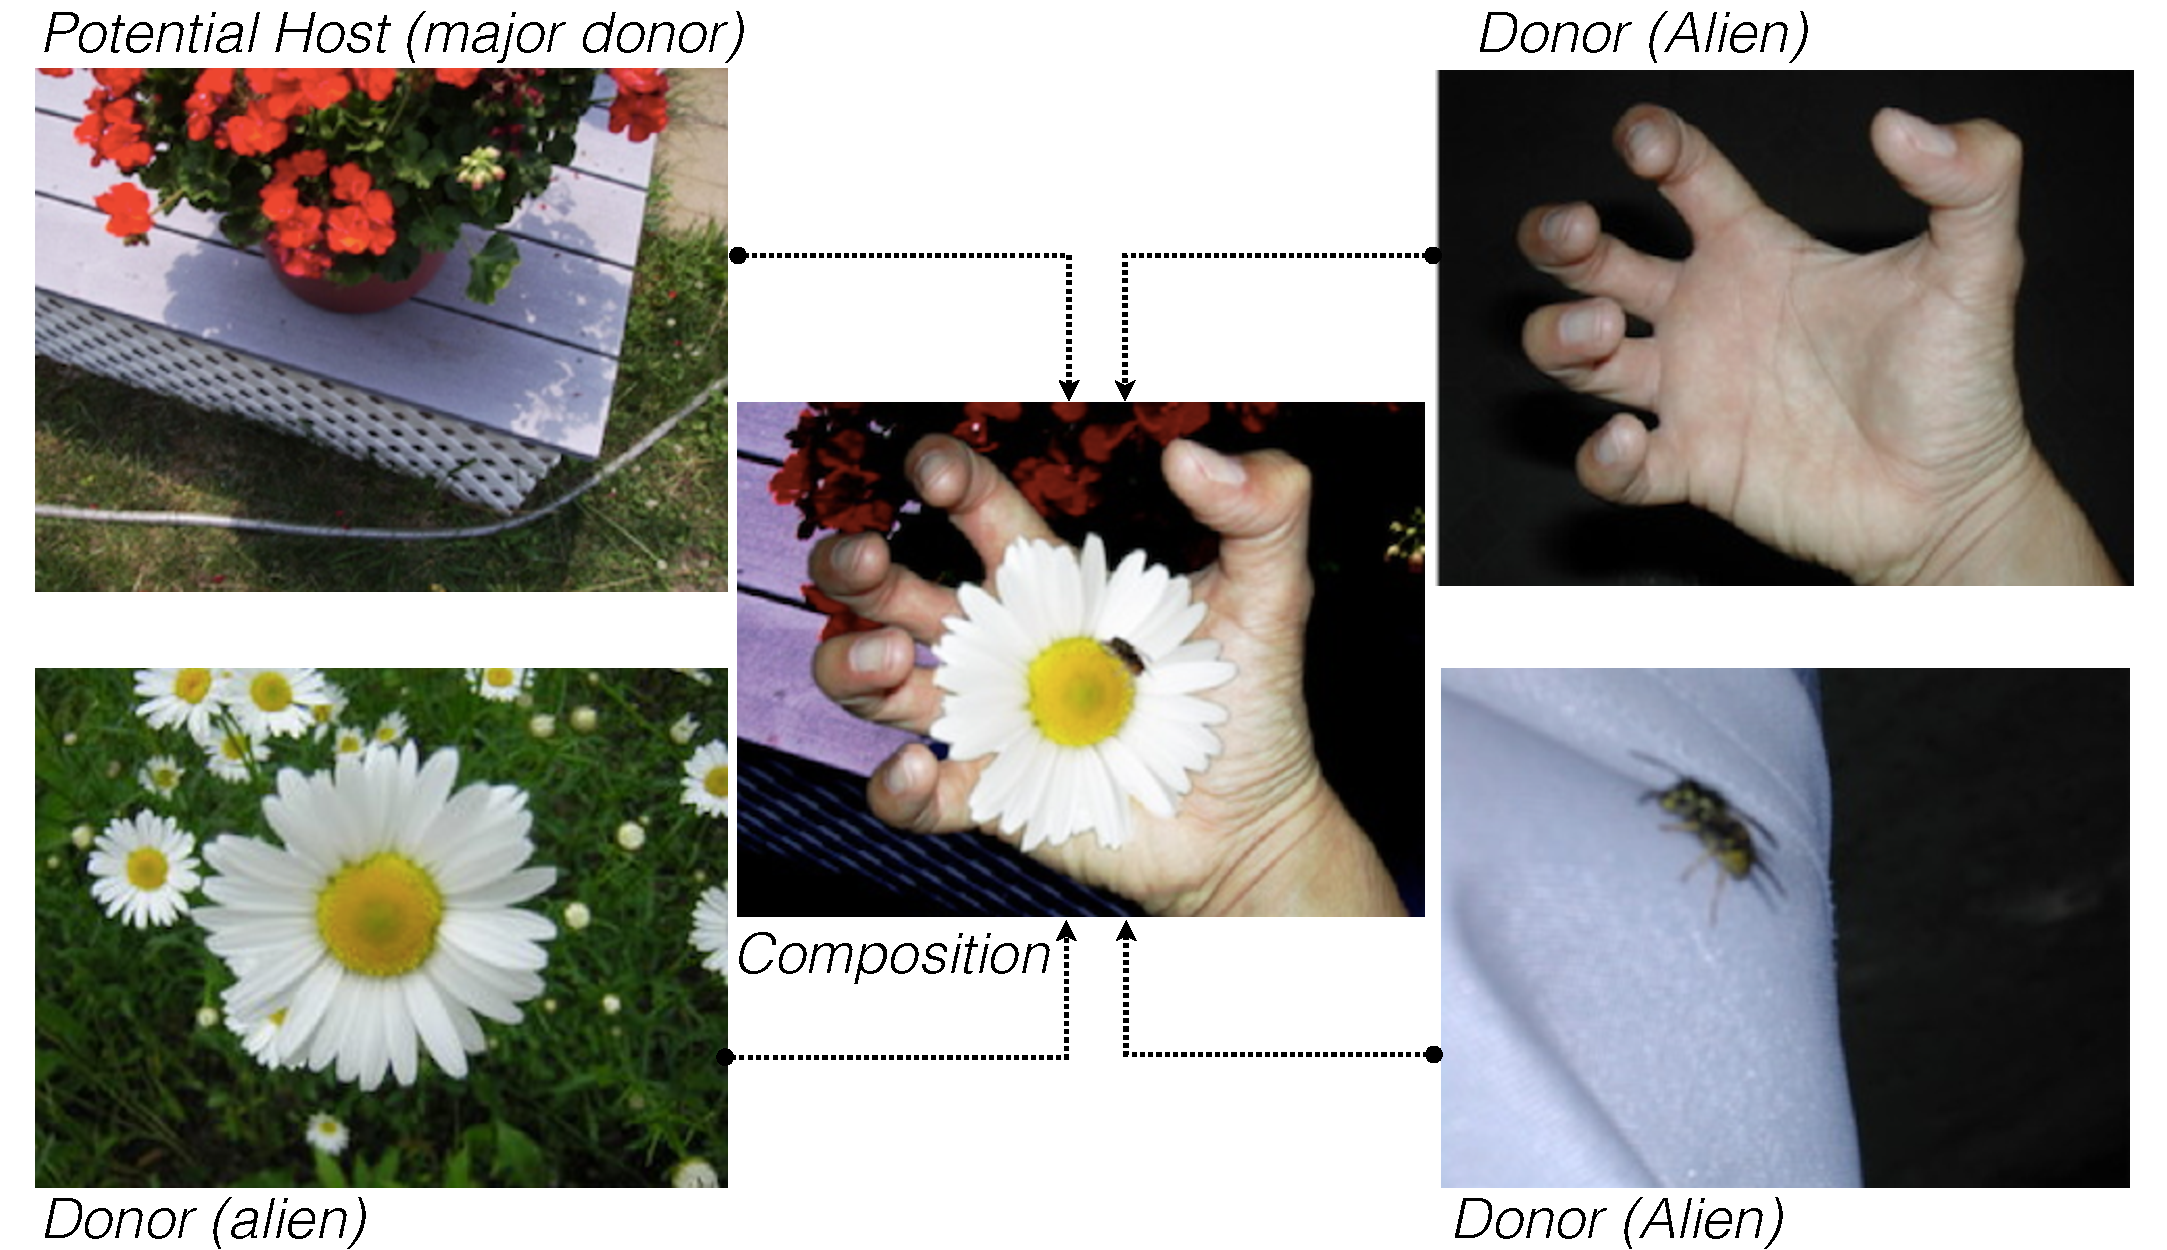
\includegraphics[width=0.67\columnwidth]{montage-provenance-filtering-02}
	}
	\caption{Contrasting multimedia phylogeny applied to near duplicate images (a) and image composites with several donors (b). While the former focuses on finding relationships among images that have similar overall context, the latter aims at finding the genealogy of an asset, including all possible near duplicates of the composition itself and of its donors. Example in (a) from~\cite{Dias_2013}; example in (b) from the NIST Nimble 2016 dataset~\cite{Nimble_2016}.}
	\label{fig:fig1}
	\end{center}
\end{figure}

%After important breakthroughs in digital forensics in the past 20 years, recent advances in machine learning and computer vision are pushing some of the research in this area to more challenging endeavors. 

Rather than focusing on checking the integrity of a single multimedia object (as it used to be with most of the proposed methods from the early 2000s until recently), some researchers in digital forensics are now seeking to leverage all possible information associated to a pool of objects, analyzing their space and time relationships. Such recent efforts are made possible by a research field known as Multimedia Phylogeny~\cite{Dias_2012,Dias_2013} --- a relatively new discipline that studies the evolutionary processes that influence multimedia objects and collections, as well as the relationship among transformed versions of an object, looking for causal and ancestry relationships, the types of transformations, and the order in which they were applied to objects. 

Such new developments are necessary in order to adapt forensics methods to a rapidly evolving society. The increasingly frequent occurrence of image and video compositions on the Internet and social media render the applications of phylogeny very useful in practical scenarios such as content tracking, forensics and copyright enforcement~\cite{Dias_2012,Dias_2013}. Within this new reality, forensics analysts are interested not only in determining if a digital object is fake or real but also in pinpointing who created it, what happened, when and how (genealogy) an asset was created. This process might be of significant importance in the era of post-truth~\cite{Keyes_2004,Mahler_2016,Schulten_2017} for determining how a composition was crafted, what parts went into creating the composite, and whether there was re-staging, re-purposing or an overall change of semantics~\cite{Rocha:CSUR:2011}. 

Nonetheless, before analyzing a pool of objects looking for possible kinship relationships, we need to be able to comb through large quantities of data looking for the very pieces potentially associated with a given query $q$. This task needs to be performed prior to subsequent multimedia phylogeny steps --- namely the pairwise image dissimilarity calculations and the phylogenetic graph analysis and construction --- and it is referred to herein as \emph{provenance filtering}. 

Most of the work thus far in multimedia phylogeny has overlooked the provenance filtering task, considering it to be a reasonably well solved problem~\cite{Dias_2012,Dias_2013}. The rationale behind that assumption was that most phylogeny works focused on finding the evolutionary processes associated with near-duplicate~\cite{Dias_2012} and semantically-similar images~\cite{Dias_2013}. In both setups, original images may undergo transformations over time but cannot have their overall semantics changed. 
When we consider forged and composite images, we bring new elements to the table. In this case, we now have the appearance of multiple parenting phylogeny~\cite{Oliveira_2016}, a setup in which an image might be the composite result of several other images, each with its own evolutionary chain of modifications. The composite image itself might also have its own chain of descendants and so on. Fig.~\ref{provenance_nndr} shows an example of semantically-similar images in which an original image might undergo several transformations and generate offspring. Each child can also generate others. However, the transformations tend to keep the overall meaning of the scene. In turn, as we see in Fig.~\ref{provenance_mpp}, an image in a multiple parenting setup might be the result of combining several others, each of which having its own chain of ancestors and descendants. 

Near-duplicate detection (NDD) methods~\cite{Ke_2004,Zhou:MM:2010,Tang:ICIP:2015,Yuan:ICIP:2015, Zeng:ICIP:2016} work properly for the task of finding semantically-similar images (Fig.~\ref{provenance_nndr}), upon which phylogeny graph construction algorithms could operate later on. However, NDD methods might fail in the presence of multiple donors (Fig.\ref{provenance_mpp}) given that the context and meaning of each donor is too diverse to be represented and captured by current methods. Moreover, each donor might undergo several transformations in the composition creation process including color, geometric, and affine operations. For those cases, even partial near-duplicate detection methods could fail~\cite{Dong:ICMR:2012}. Likewise, traditional content-based image retrieval (CBIR) methods~\cite{Datta_2008} would not work directly either as they often aim to determine the overall meaning of the scene and its generalization to provide the user with similar images respecting the principles of novelty and diversity~\cite{Deselaers_2009}. 

While related work for multimedia phylogeny abounds, prior work on  provenance filtering is almost non-existent. In terms of phylogeny, Dias et al.~\cite{Dias_2012} presented a minimum spanning tree-based algorithm to find a directed graph that represented the phylogeny tree of a group of near-duplicate images. This work was extended to deal with images from multiple cameras and their near duplicates~\cite{Dias_2013}. Other media have also been considered such as videos~\cite{Dias_2011,Lameri_2014}, audio~\cite{Nucci_2013} and text~\cite{Andrews_2012}. Oliveira~et~al.~\cite{Oliveira_2016} extended the image phylogeny formulation to deal with multiple donors and descendants simultaneously more aligned with the context of this paper. However, their work assumes the candidate images are known a priori.  

Important advances have been made on finding ancestral relationships between pairs of images; nevertheless, the performance of such algorithms is significantly degraded if a good set of potentially related images is not found beforehand. In this vein, we extend upon image representation and indexing techniques (common in NDD and CBIR areas) to deal with provenance filtering for multiple donor and composite images. Our technique comprises two stages: in the first, we query an image collection for the most likely donors that might have contributed to the creation of the query, if it is a composite. This is done following a traditional CBIR pipeline, which involves image representation through appropriate features and the adoption of a subsequent indexing mechanism (more details in Sec.~\ref{sec:method}). The top retrieved results are then analyzed and compared to the query using scale and rotation-invariant points of interest~\cite{Bay:CVIU:2008}, nearest neighbor distance ratio policy~\cite{Lowe_1999}, and geometric alignment~\cite{Zitova_2003}. After finding the best possible match to the query, we use that image along with the query to calculate a contextual mask to serve as an activation of possible regions that are different between them. Such regions are candidate regions for possible donors. We then proceed with the second stage of the search, querying the collection for images that are similar to the selected regions of interest in the query as pointed out by the contextual mask. Ultimately, we aggregate the different rankings to create a final ranked list of images related to the query in terms of possible donors contributing to its creation process and thus closing the loop for provenance filtering.

The contributions of this work are (i) the exploration of different querying and indexing techniques for the new problem of provenance filtering; (ii) the incorporation of provenance context to single out possible candidate regions related to donors in the creation processo of a query; and (iii) the study of the efficiency and effectiveness tradeoffs involved in the provenance filtering task while dealing with very large collections of images. 

%We organized the remaining of this paper into three sections. Sec.~\ref{sec:method} presents the proposed methodology, decisions and setup while Sec.~\ref{sec:experiments} shows the performed experiments for a provenance dataset provided by the National Institute of Standards and Technology (NIST) and RankOne Inc. comprising more than one million images. Finally, Sec.~\ref{sec:conclusions} concludes this work and sheds light on possible future work along with the integration of provenance filtering with  the more general multimedia phylogeny problem. 

